\subsection{Gated feedback recurrent neural networks}

\textit{Gated feedback recurrent neural networks} were proposed in 2015 by  Chung et al. \cite{gatedFeedback} as a novel recurrent network architecture.
Unlike LSTM or GRU where the novelty of the proposal was a new kind of unit, designed to better capture long-term dependencies between inputs, the novelty of this approach is the way the units are arranged. For starters multiple recurrent layer are used, like in a \textit{Stacked RNN}, i.e. the network is composed of several layers, each one of which is connected to all the others; in other words the layers are fully connected. Moreover, unlike traditional stacked RNNs, the feedback connection between different layers is gated by a \textit{global reset gate} which is essentially a logistic unit computed on the current inputs and the previous states of hidden layers. This global reset gates is reminiscent of the gates of LSTM and GRU but it controls the connection between layers not between units: the hidden state values of layer $i$ at time $t-1$ are fed to a lower layer $j$ multiplied by $g^{i\rightarrow j}$.
The gate between layers $i$ and $j$ is computed as:
\begin{equation}
g^{i\rightarrow j} \defeq \sigma(\vec{w}_g^{i\rightarrow j} \cdot \vec{h_t}^{j-1} + \vec{u}_g^{i\rightarrow j} \cdot \vec{h}^*_{t-1})
\end{equation}
where $\vec{w}_g^{i\rightarrow j}$ and $\vec{u}_g^{i\rightarrow j}$ are the weights of the links between the gate and the input and the hidden states of all layers at time-step $t-1$ respectively; for $j=1$,  $\vec{h}_t^{j-1}=\vec{x}_t $  and $\vec{h^*_{t-1}}$ represents all the hidden states at time $t-1$.

The idea behind this architecture is to encourage each recurrent layer to work at different timescales, hence capturing both long-term and short-term dependencies. In addition, the units composing the layers, can be traditional sigmoidal units but also LSTM or GRU, hence benefiting from both the strength of these kind of units and the global gate mechanism. In \cite{gatedFeedback} the architecture is evaluated against traditional and stacked RNNs with both LSTM and GRU units: gated feedback networks are shown to offer better performance and accuracy in several challenging tasks.


\tikzstyle{rnn_style}=[->,shorten >=1pt,auto,node distance=1.5cm,
  thick,
  neuron/.style={circle,fill=white!50,draw,node distance = 1cm, minimum size=0.7cm,font=\sffamily\Large\bfseries},
  gate/.style={circle,fill=white!50,draw,node distance = 1cm,font=\sffamily\small\bfseries},
  missing/.style={rectangle,fill=white!50,node distance =1cm,draw=none,minimum size=0.7cm,font=\sffamily\Huge\bfseries},
  label/.style={node distance=1.2cm,rectangle,fill=white!50,draw=none,minimum size=0.7cm,font=\sffamily\normalsize},
  layer/.style={rectangle,fill=white!50,draw,minimum width=4cm,minimum height=0.5cm, font=\sffamily\normalsize},
  gateEdge/.style={dotted},]
\begin{figure}
 \centering
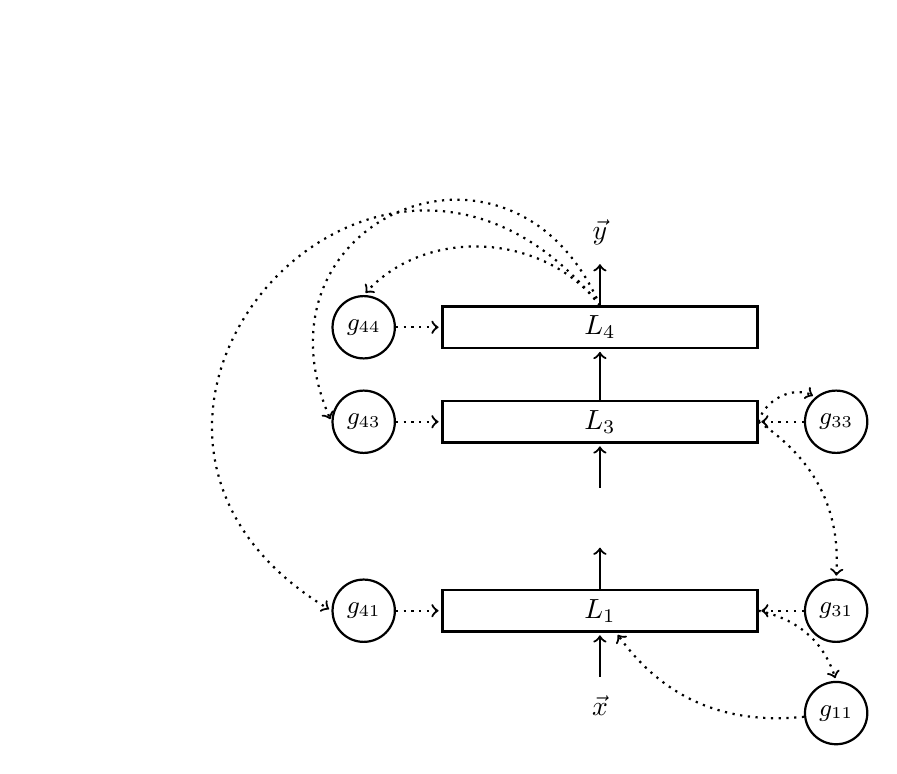
\begin{tikzpicture}[rnn_style]
  
  \node[layer] (l1)[] {$L_1$};
  \node[missing] (l2)[above of=l1,node distance=1.2cm]{$\hdots$};
  \node[layer] (l3)[above of=l2,node distance=1.2cm] {$L_3$};
  \node[layer] (l4)[above of=l3,node distance=1.2cm] {$L_4$};
  
  \node[label] (x) [below of=l1, node distance=1.2cm]{$\vec{x}$};
  \node[label] (y) [above of=l4, node distance=1.2cm]{$\vec{y}$};

  
    \path[->] (l1) edge 	[] node[]{}   	(l2)
	    (l2) edge 	[]   		(l3)
	    (l3) edge	[]		(l4)
	    (x) edge[]			(l1)
	    (l4) edge[]			(y);
  
  \node[gate] (g44)[left of=l4, node distance =3cm]{$g_{44}$};
  \node[gate] (g43)[left of=l3, node distance =3cm]{$g_{43}$};
  \node[gate] (g41)[left of=l1, node distance =3cm]{$g_{41}$};
  \node[gate] (g33)[right of=l3, node distance =3cm]{$g_{33}$};
  \node[gate] (g31)[right of=l1, node distance =3cm]{$g_{31}$};
  \node[gate] (g11)[below of=g31, node distance =1.3cm]{$g_{11}$};
  
      \path[->] (g44) edge[gateEdge]   		(l4)
		(l4.north)  edge[gateEdge,bend right=50] (g44.north)
		(l4.north)  edge[gateEdge,bend right=90,distance=2.8cm] (g43.west)
		(g43) edge[gateEdge]		(l3)
		(l4.north)  edge[gateEdge,bend right=100, distance =4.5cm] (g41.west)
		(g41) edge[gateEdge]		(l1)
		(l3.east)  edge[gateEdge,bend left=50, anchor=east]	(g33)
		(g33) edge[gateEdge]		(l3)
		(l3.east)  edge[gateEdge,bend left]	(g31.north)
		(g31) edge[gateEdge]		(l1)
		(l1.east) edge[gateEdge, bend left]		(g11.north)
		(g11) edge[gateEdge, bend left]		(l1);

\end{tikzpicture}
\caption{Gated feedback architecture. Only connections between layers are shown, dotted when trough gates.}
\label{fig:gated}
\end{figure}

